% \iffalse
\let\negmedspace\undefined
\let\negthickspace\undefined
\documentclass[journal,12pt,twocolumn]{IEEEtran}
\usepackage{cite}
\usepackage{amsmath,amssymb,amsfonts,amsthm}
\usepackage{algorithmic}
\usepackage{graphicx}
\usepackage{textcomp}
\usepackage{xcolor}
\usepackage{txfonts}
\usepackage{listings}
\usepackage{enumitem}
\usepackage{mathtools}
\usepackage{float}
\usepackage{gensymb}
\usepackage{comment}
\usepackage[breaklinks=true]{hyperref}
\usepackage{tkz-euclide} 
\usepackage{listings}
\usepackage{gvv}                                        
\def\inputGnumericTable{}                                 
\usepackage[latin1]{inputenc}                                
\usepackage{color}                                            
\usepackage{array}          
\usetikzlibrary{positioning, arrows.meta}
\usepackage{longtable}                                       
\usepackage{calc}                                             
\usepackage{multirow}                                         
\usepackage{hhline}                                           
\usepackage{ifthen}                                           
\usepackage{lscape}
\usepackage{amsmath}
\newtheorem{theorem}{Theorem}[section]
\newtheorem{problem}{Problem}
\newtheorem{proposition}{Proposition}[section]
\newtheorem{lemma}{Lemma}[section]
\newtheorem{corollary}[theorem]{Corollary}
\newtheorem{example}{Example}[section]
\newtheorem{definition}[problem]{Definition}
\newcommand{\BEQA}{\begin{eqnarray}}
\newcommand{\EEQA}{\end{eqnarray}}
\newcommand{\define}{\stackrel{\triangle}{=}}
\theoremstyle{remark}
\newtheorem{rem}{Remark}
\begin{document}

\bibliographystyle{IEEEtran}
\title{GATE-EE-Q14}
\author{EE23BTECH11015 - DHANUSH V NAYAK$^{*}$% <-this % stops a space
}
\maketitle
\newpage
\bigskip
\renewcommand{\thefigure}{\arabic{figure}}
\renewcommand{\thetable}{\theenumi}
\textbf{Question:}Consider a unity-gain negative feedback system consisting of the plant $G\brak{s}$  and a proportional-integral controller. Let the proportional gain and integral
gain be 3 and 1, respectively. For a unit step reference input, the final values of the
controller output and the plant output, respectively, are
\begin{align}
    G\brak{s} = \frac{1}{\brak{s-1}} \notag
\end{align}
\solution 
\begin{table}[H]
\centering
\renewcommand\thetable{1}
\setlength{\extrarowheight}{9pt}
\resizebox{0.5\textwidth}{!}{
\begin{tabular}{|c|c|c|}
\hline
\textbf{Parameter} & \textbf{Description} & \textbf{Value} \\ \hline
$K_{p}$ & Proportional Gain & 3  \\ \hline
$K_{i}$ & Integral Gain &1 \\ \hline
$r\brak{t}$& Reference Input & $u\brak{t}$ \\ \hline 
$w\brak{t}$& Controller Output & $?$ \\ \hline 
$y\brak{t}$ & Plant Output & $?$ \\ \hline
$F\brak{s}$ & Feedback Gain & $1$ \\ \hline
$C\brak{s}$ & Controller Gain & $3+\frac{1}{s}$ \\ \hline
$e\brak{t}$ & Error Input & $r\brak{t}-y\brak{t}$ \\ \hline
\end{tabular}}
\caption{Parameter Table}
\label{tab:gate_ee_Q14}
\end{table}

From the\figref{fig:gate_ee_Q14_blockdiagram}:
\begin{align}
    E\brak{s}&= U\brak{s} - Y\brak{s}\\
             &= \frac{1}{s} - Y\brak{s}\label{eq:gate_ee_Q14.1}
\end{align}
Also,
\begin{align}
    W\brak{s} &= 3E\brak{s} + \frac{1}{s}E\brak{s}\label{eq:gate_ee_Q14.2}
\end{align}
From equation \eqref{eq:gate_ee_Q14.1} :
\begin{align}
    W\brak{s} &= \frac{3}{s} + \frac{1}{s^2} - Y\brak{s}\brak{3+\frac{1}{s}}\label{eq:gate_ee_Q14.3}
\end{align}
\begin{figure}[H]
    \resizebox{0.55\textwidth}{!}{
\tikzset{
    block/.style = {draw, fill=white, rectangle, minimum height=3em, minimum width=3em},
    tmp/.style  = {coordinate}, 
    sum/.style= {draw, fill=white, circle, node distance=1cm},
    input/.style = {coordinate},
    output/.style= {coordinate},
    pinstyle/.style = {pin edge={to-,thin,black}}
}


\begin{tikzpicture}[auto, node distance=2cm,>=latex']
    \node [input, name=rinput] (rinput) {};
    \node [sum, right of=rinput] (sum1) {};
    
    
    \node [block, right of=sum1] (controller) {$k_{p}=3$};
    \node [block, above of=controller, node distance=2cm] (up) {$\frac{k_{i}}{s}=\frac{3}{s}$};
    
    \node [sum, right of=controller, node distance=2cm] (sum2) {};
    % Removed the block labeled "αβ2"
    \node [block, right of=sum2, node distance=3cm] (system) {$G\brak{s}=\frac{1}{\brak{s-1}}$};
    \node [output, right of=system, node distance=2cm] (output) {};
    \node [tmp, below of=controller] (tmp1) {$H(s)$};

    \draw [->] (rinput) -- node{$r\brak{t}$} (sum1);
    \draw [->] (sum1) -- node[name=z,anchor=north]{$e\brak{t}$} (controller);
    \draw [->] (controller) -- (sum2);
    \draw [->] (sum2) -- node{$w\brak{t}$} (system);
    \draw [->] (system) -- node [name=y] {$y\brak{t}$} (output);
    \draw [->] (z) |- (up);
    \draw [->] (up) -| (sum2);
    \draw [->] (y) |- (tmp1) -| node[pos=0.99] {$-$} (sum1);
\end{tikzpicture}



}
    \caption{Block Diagram of System}
    \label{fig:gate_ee_Q14_blockdiagram}
\end{figure}
\begin{align}
    Y\brak{s} &= G\brak{s}W\brak{s}
\end{align}
Using equaton   \eqref{eq:gate_ee_Q14.3} and data from \tabref{tab:gate_ee_Q14}:
\begin{align}
    Y\brak{s} &=  \frac{3s+1}{s\brak{s+1}^2} ,  Re\brak{s}>-1 \label{eq:Y(s)}
\end{align}
Substituting equation\eqref{eq:Y(s)} in equation \eqref{eq:gate_ee_Q14.3}:
\begin{align}
    W\brak{s} &= \frac{\brak{s-1}\brak{3s+1}}{s\brak{s+1}^2} ,  Re\brak{s}>-1 \label{eq:W(s)}
\end{align}
Final Value Theorem:    
\begin{align}
    \lim_{t \to \infty} x\brak{t}&= \lim_{s \to 0} sX\brak{s}\label{eq:gate_ee_Q14.4}
\end{align}
Applying Final Value Theorem on Y\brak{s}:
\begin{align}
     \lim_{t \to \infty} y\brak{t}&= \lim_{s \to 0} sY\brak{s}\\
                            &= 1
\end{align}
Applying Final Value Theorem on W\brak{s}:
\begin{align}
     \lim_{t \to \infty} w\brak{t}&= \lim_{s \to 0} sW\brak{s}\\
                            &= -1
\end{align}
Taking partial fraction of equation\eqref{eq:Y(s)} :
\begin{align}
    Y\brak{s} &= \frac{1}{s} + \frac{2}{\brak{s+1}^2} - \frac{1}{s+1}
\end{align}
\begin{align}
    tx\brak{t} &\system{L} -\frac{d{X\brak{s}}}{ds} \label{eq:laplace_diff_prop}\\
    e^{-at}x\brak{t} &\system{L} X\brak{s+a}\label{eq:laplace_timeshifting_prop}
\end{align}
By using equation \eqref{eq:laplace_diff_prop} and \eqref{eq:laplace_timeshifting_prop}:
\begin{align}
    e^{-t}u\brak{t} &\system{L} \frac{1}{s+1} ,  Re\brak{s}>-1 \label{eq:gate_ee_Q14result.1}\\
    t e^{-t}u\brak{t} &\system{L} \frac{1}{\brak{s+1}^2},  Re\brak{s}>-1 
 \label{eq:gate_ee_Q14result.2}
\end{align}
\begin{align}
    \therefore y\brak{t} &= u\brak{t}+ 2t e^{-t}u\brak{t} - e^{-t}u\brak{t}
\end{align}
Taking partial fraction of equation\eqref{eq:W(s)} :
\begin{align}
    W\brak{s} &= -\frac{1}{s} - \frac{4}{\brak{s+1}^2} + \frac{4}{s+1}
\end{align}
Using equations \eqref{eq:gate_ee_Q14result.1} and \eqref{eq:gate_ee_Q14result.2} and taking inverse lapalace transform:
\begin{align}
    w\brak{t} &= -u\brak{t}-4t e^{-t}u\brak{t} +4 e^{-t}u\brak{t}
\end{align}
\begin{figure}[H]
    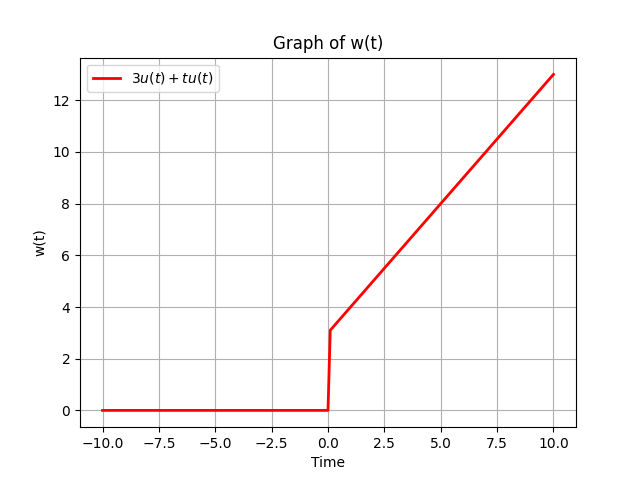
\includegraphics[width=1\columnwidth]{figs/Plot of w(t).png}
    \caption{Plot of $w\brak{t}$}
    \label{fig:w_t}
\end{figure}

\begin{figure}[H]
    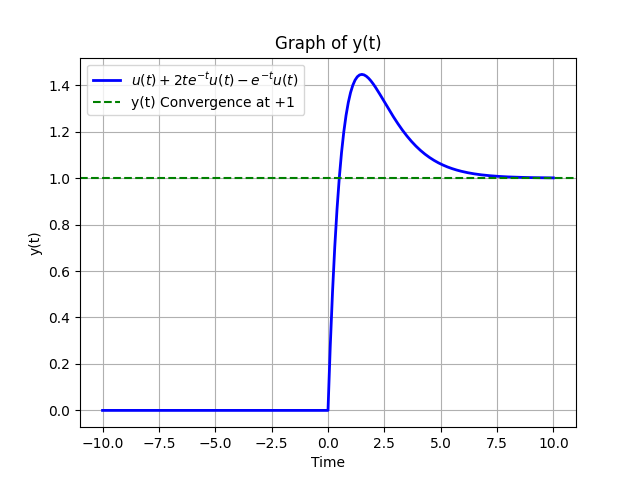
\includegraphics[width=1\columnwidth]{figs/Plot of y(t).png}
    \caption{Plot of $y\brak{t}$}
    \label{fig:y_t}
\end{figure}

From the graph also its clear that finally $w\brak{t}$ approach $-1$ and $y\brak{t}$ approach $1$ .
\end{document}

